\documentclass[a4paper,12pt]{report}

\usepackage{alltt, fancyvrb, url}
\usepackage{graphicx}
\usepackage[utf8]{inputenc}
\usepackage{float}
\usepackage{hyperref}

% Questo commentalo se vuoi scrivere in inglese.
\usepackage[italian]{babel}

\usepackage[italian]{cleveref}

\title{Relazione \\``Time2Survive''}

\author{Andrea Cecchini \\ Nicolò D'Addabbo \\ Luca Oskari Fiumanò \\Leonardo David Matteo Magnani}
\date{\today}


\begin{document}

\maketitle

\tableofcontents

\chapter{Analisi}

\section{Requisiti}
Il progetto si pone l’obiettivo di creare un videogioco survival shoot ‘em up ispirato a ``The Binding of Isaac'' \footnote{\url{https://store.steampowered.com/app/113200/The_Binding_of_Isaac/}}.
Con survival shoot ‘em up si intende un genere di videogioco nella quale l’obiettivo è sopravvivere il più a lungo possibile a ondate di nemici, generandone di nuove una volta eliminata la precedente.

\subsection*{Requisiti funzionali}
\subsubsection{Requisiti Funzionali Obbligatori}
\begin{itemize}
	\item Il gioco dovrà occuparsi di gestire la partita dell’utente all’interno della mappa di gioco di Time2Survive, rendendo più difficile la sopravvivenza del giocatore attraverso ondate di nemici di difficoltà crescente.
    All’interno della mappa, il giocatore potrà:
    \begin{itemize}
        \item Sfruttare le proprie abilita’ di videogiocatore per sopravvivere alle numerose ondate dei nemici che si susseguiranno.
        \item Sfidare ondate che verranno generate al completamento della precedente. Le ondate terminano quando tutti i nemici sono stati eliminati.
        \item I nemici si potranno eliminare attraverso l'utilizzo di proiettili generati dal personaggio.
        \item La partita sarà conclusa alla morte virtuale del giocatore.
    \end{itemize}
	\item Il giocatore si troverà all'interno di una stanza in cui verranno generate le ondate di nemici.
	\item La difficoltà del gioco sarà incrementale e riguarderà sopratutto le ondate. Essa sarà manipolata attraverso 3 parametri:
    \begin{itemize}
        \item Numero: numero dei nemici a schermo.
        \item Resilienza: resistenza agli attacchi da parte del giocatore.
        \item Forza: danno provocato dal nemico.
    \end{itemize}
	\item Il giocatore si potrà muovere nell’ambiente di gioco costituito da una singola stanza.
    \item I nemici sono delle entità attive del gioco che cercano di eliminare il giocatore.
    Vengono controllati da una semplice AI (Artificial Intelligence). 
	Per intelligenza artificiale si intende un software che conferisce a ogni nemico una strategia di movimento e di combattimento.
    \item Il giocatore dovrà essere in grado di capire lo stato della partita in ogni momento della suddetta visualizzando la propria vita. 
	Il giocatore sarà inoltre in grado di visualizzare le proprie capacità essendo in grado di visualizzare il numero di ondate alle quali è sopravvissuto.
\end{itemize}

\subsubsection{Requisiti Funzionali Opzionali}
\begin{itemize}
	\item Per aiutare il giocatore, saranno disponibili diversi potenziamenti che gli permetteranno di aumentare le proprie abilità.
	\item Per rendere più vario la partita saranno presenti diversi tipi di nemici con caratteristiche uniche e diverse tra loro.
\end{itemize}
\subsection*{Requisiti non funzionali}
\begin{itemize}
	\item 
\end{itemize}
\newpage
\section{Analisi e modello del dominio}
T2S mette a disposizione del giocatore la possibilità di giocare una nuova partita.
\\
Una partita gestisce il proprio stato e il mondo di gioco di T2S.
\\
Il mondo di T2S è l’arena dove le diverse entità interagiscono fra di loro.
\\
Al giocatore sarà data la possibilità di controllare una di queste entità, il quale sarà l’avatar del giocatore nella partita.
\\
Durante lo svolgimento della partita verranno generate delle ondate di entità controllate da un’intelligenza artificiale con il compito di attaccare e uccidere l’avatar del giocatore.
\\
Per combattere questi nemici, l’avatar avrà la possibilità di sparare dei proiettili che possono essere migliorati tramite potenziamenti.
\\
Una volta sconfitta un’ondata viene aggiornato lo stato della partita incrementando il numero di round alla quale si è sopravvissuti e viene generata una nuova ondata di maggiore difficoltà.
\\
All’inizio della partita all’avatar verranno assegnati dei proiettili di default e un determinato numero di punti vita.
\\
Una volta subito un danno, a seconda della sua entità, verrà detratta una certa quantità dalla vita corrente.
\\
La partita termina quando il giocatore ha perso tutti i suoi punti vita.
\\
Le difficoltà che il progetto si porta dietro sono:
\begin{itemize}
	\item Un’implementazione di un intelligenza artificiale in grado di controllare correttamente i nemici. La prima versione del gioco fornirà ai nemici un Controller basato sulle coordinate del player nella mappa. 
	\item Una grafica completa che verrà implementata inizialmente in maniera minimale.

\end{itemize}

\begin{figure}[H]
\centering{}
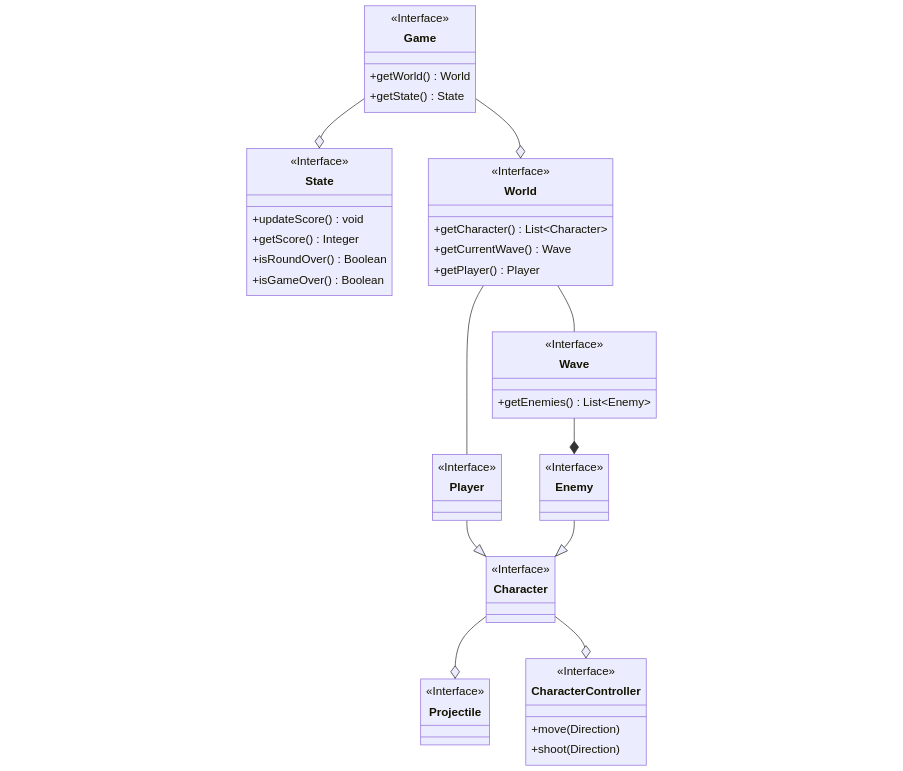
\includegraphics[width=1\textwidth]{img/Schema-UML-Analisi.png}
\caption{Schema UML dell'analisi del problema, con rappresentate le entità principali ed i rapporti fra loro}
\label{img:analysis}
\end{figure}




\chapter{Design}
\section{Architettura}
T2S è stato sviluppato adottando un pattern architetturale che mantenesse una simile struttura MVC, quindi con i suoi vantaggi, contaminandola però attraverso l’utilizzo del pattern Component.
\\
Il pattern Component permette ad una singola entità di estendersi su domini multipli senza accorparli in unica classe.
\\
Applicandolo al dominio dell’applicazione (Model), avremo che ogni entità risulta essere un GameObject.
\\
Tale GameObject viene adornato con dei GameComponent, ognuno dei quali appartiene ad un dominio (Input,Fisica,Stato,Grafica …) particolare.
\\
Ogni GameComponent è responsabile per l’aggiornamento del GameObject nel rispettivo dominio.
\\
Tuttavia, pur appartenendo a domini diversi, i diversi GameComponents potrebbero aver bisogno di comunicare tra di loro.
\\
Sfruttando come “container” il GameObject stesso è stato messo a disposizione dei GameComponents un semplice ma funzionale sistema di messaggistica.
\\
L’utilizzo di questi componenti porta ad importanti vantaggi:
\begin{itemize}
	\item \textbf{Stroncamento di un albero di ereditarietà troppo complesso e lungo}:
	Per rappresentare entità con diversi comportamenti si utilizza la composizione di GameComponent che implementino quei comportamenti, senza nessun utilizzo dell’ereditarietà.
	%
	\item Eliminazione del problema \textbf{Deadly Diamond of Death}
	%
	\item \textbf{Riduzione al minimo delle ripetizioni di codice} dovuto alla creazione di componenti altamente riutilizzabili
\end{itemize}
Dal punto di vista del pattern architetturale Model-View-Controller, i rispettivi moduli sono rappresentati da:
\begin{itemize}
	\item \textbf{Model}:
	Viene seguito il seguente mantra “Everything is a GameObject”		
Difatti ogni entità del dominio viene rappresentata e astratta grazie all’utilizzo 	dell’interfaccia GameObject, la quale svolge il ruolo di “container” di GameComponents.
	%
	\item \textbf{Controller}:
 Questo ruolo viene affidato all’interfaccia GameEngine, la quale ha il compito di gestire l’aggiornamento di ogni GameObject e dei suoi componenti e la renderizzazione sulla View.
	%
	\item \textbf{View}:
 Il ruolo della view viene demandato a due interfacce ben connesse tra di loro: Scene  e Graphics.
L’interfaccia Scene astrae il concetto di “Scena” di gioco
L’interfaccia Graphics ha il compito di saper “disegnare” i diversi GameObjects con la 
tecnologia grafica dipesa dall’implementazione e fornita dall'implementazione di Scene.
\end{itemize}
Dal diagramma delle classi, qui sotto fornito, è possibile notare un elemento di differenza rispetto ad una classica architettura MVC: un componente di spicco,denominato GraphicsComponent, risulta avere dei riferimenti alla parte di view e di model, creando un collegamento che a prima vista potrebbe risultare problematico.
%
La modularità di M.V.C. non viene però attaccata: volendo, come esempio, cambiare la tecnologia di sviluppo per quanto riguarda la grafica si modificherà esclusivamente la parte di View dell'applicazione, senza ripercussioni in nessun altro modulo del programma.
%
L’ipotetico passaggio da JavaFx e Swing, dunque, non risulta essere problematico: 
%
si dovranno sostituire le implementazioni di JavaFx delle interfacce Graphics e Scene con delle nuove implementazioni che utilizzino Swing.

\begin{figure}[H]
\centering{}
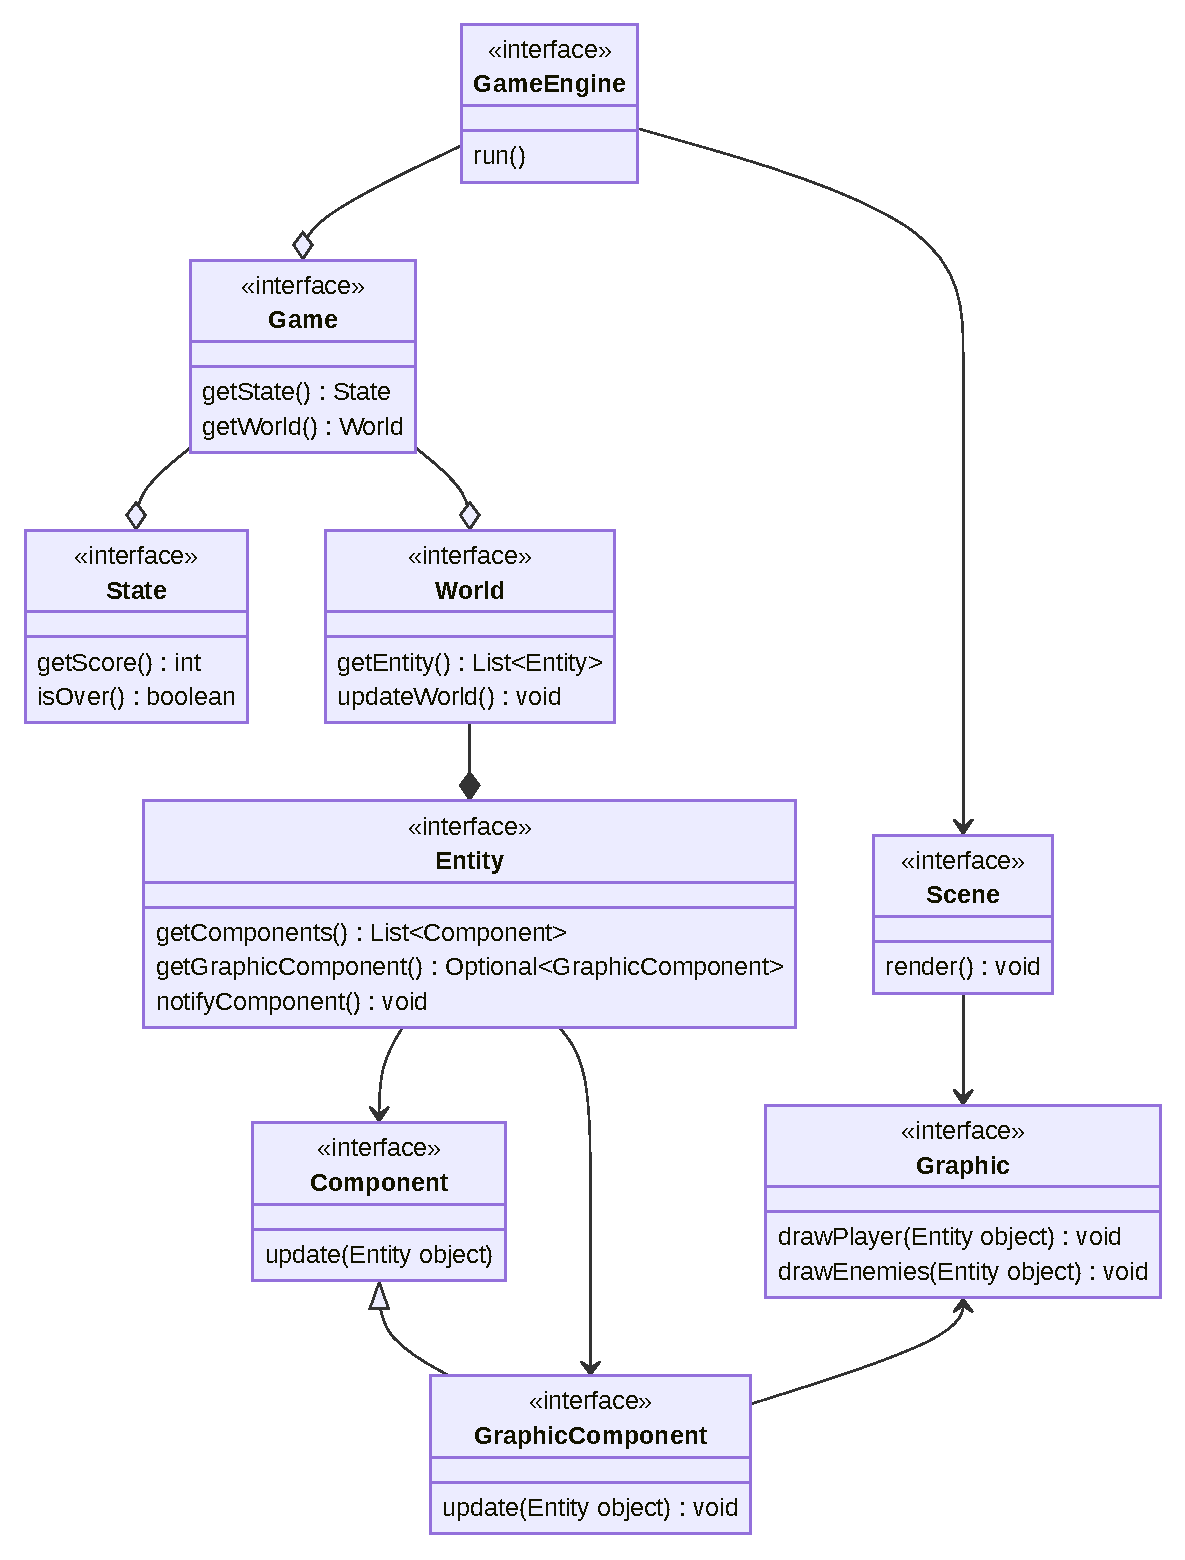
\includegraphics[width=1\textwidth]{img/SoftwareArchitectureUML.pdf}
\caption{Schema UML architetturale di T2S.}
\label{img:analysis}
\end{figure}

\section{Design dettagliato}

\subsection*{Nicolò D'Addabbo}

\subsubsection{Input Controller intercambiabili}

\begin{figure}[H]
\centering{}
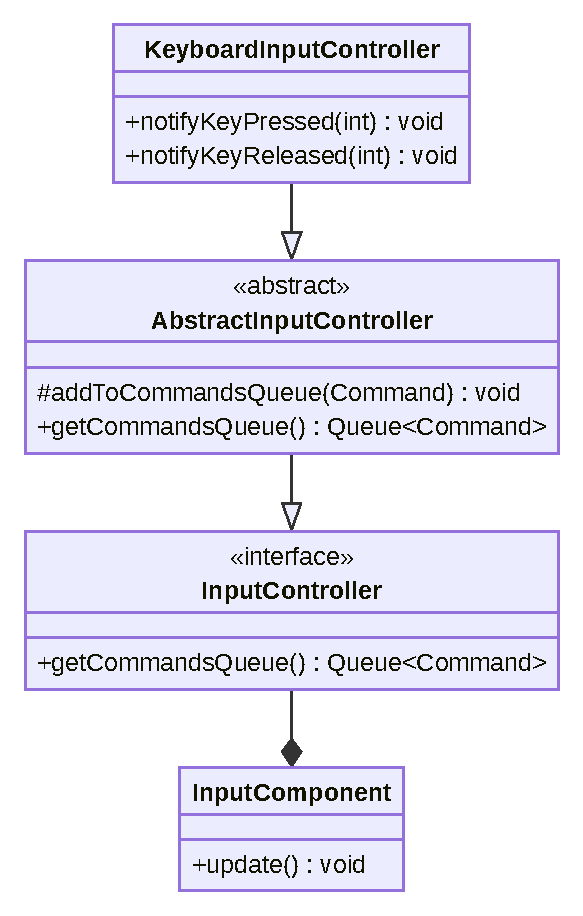
\includegraphics[scale=0.75]{img/InputControllerUML}
\caption{Rappresentazione UML del pattern Strategy per l'Input Component}
\label{img:strategy}
\end{figure}

\paragraph{Problema} Un’entità può ricevere input da diverse sorgenti come ad esempio una tastiera o un joypad, 
la cui presenza non è di interesse dell’entità stessa. 
Infatti deve possedere solo un generico Input Component con un metodo update.

\paragraph{Soluzione} La classe \textbf{InputComponent} implementa lo \textit{Strategy pattern}, contenendo un riferimento a un \textit{InputController} che funge da strategia per la gestione dell'input. Quest'ultimo può essere sostituito con un'implementazione diversa, permettendo l'utilizzo di strategie differenti.
\\
Il metodo \textit{update} dell’Input Component chiama il metodo \textit{execute} su ogni \textit{Command} (come descritto nella sezione "Gestione dei comandi di gioco") presente nella coda di comandi restituita dall'\textit{InputController} (come descritto nella sezione "Input Controller con molteplici stati").
\\
Inoltre, grazie allo \textit{Strategy pattern}, è possibile sviluppare un'intelligenza artificiale in modo semplice. Un'AI, infatti, non è altro che un \textit{InputController} che genera diversi \textit{Command} in base a un determinato algoritmo.
\\

\begin{figure}[H]
\centering{}
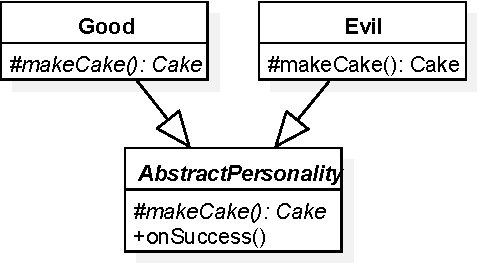
\includegraphics[width=\textwidth]{img/template}
\caption{Rappresentazione UML dell'applicazione del pattern Template Method alla gerarchia delle Personalità}
\label{img:template}
\end{figure}

\paragraph{Problema} In fase di sviluppo, sono state sviluppate due personalità, una buona ed una cattiva.
Quella buona restituisce sempre una torta vera, mentre quella cattiva restituisce sempre la
promessa di una torta che verrà in realtà disattesa.
Ci si è accorti che diverse personalità condividevano molto del comportamento,
portando a classi molto simili e a duplicazione.

\paragraph{Soluzione} Dato che le due personalità differiscono solo per il comportamento da effettuarsi in caso di percorso completato con successo,
è stato utilizzato il \textit{pattern template method} per massimizzare il riuso, come da \Cref{img:template}.
Il metodo template è \texttt{onSuccess()}, che chiama un metodo astratto e protetto
\texttt{makeCake()}.

\subsubsection{Gestione di output multipli}

\begin{figure}[H]
\centering{}
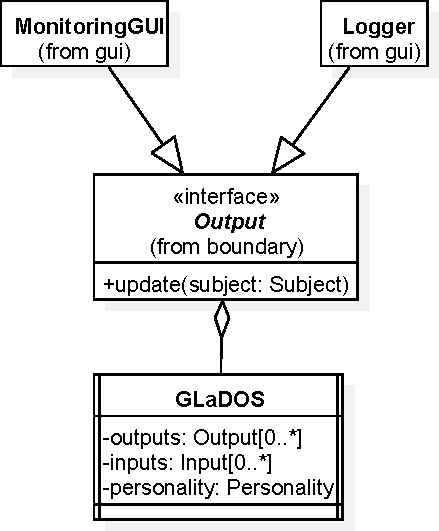
\includegraphics[width=.7\textwidth]{img/observer}
\caption{Il pattern Observer è usato per consentire a GLaDOS di informare tutti i sistemi di output in ascolto}
\label{img:observer}
\end{figure}

\paragraph{Problema} Il sistema deve supportare output multipli. In particolare, si richiede che vi sia un logger che stampa a terminale o su file,
e un'interfaccia grafica che mostri una rappresentazione grafica del sistema.

\paragraph{Soluzione} Dato che i due sistemi di reporting utilizzano le medesime informazioni, si è deciso di raggrupparli dietro l'interfaccia \texttt{Output}.
A questo punto, le due possibilità erano quelle di far sì che \texttt{GLaDOS} potesse pilotarle entrambe.
Invece di fare un sistema in cui questi output sono obbligatori e connessi, si è deciso di usare maggior flessibilità (anche in vista di future estensioni)
e di adottare una comunicazione uno-a-molti fra \texttt{GLaDOS} ed i sistemi di output.
La scelta è quindi ricaduta sul \textit{pattern Observer}: \texttt{GLaDOS} è observable, e le istanze di \texttt{Output} sono observer.
%
Il suo utilizzo è esemplificato in \Cref{img:observer}


\subsection*{Contro-esempio: pessimo diagramma UML}

In \Cref{img:badarch} è mostrato il modo \textbf{sbagliato} di fare le cose.
%
Questo schema è fatto male perché:
\begin{itemize}
	\item È caotico.
	\item È difficile da leggere e capire.
	\item Vi sono troppe classi, e non si capisce bene quali siano i rapporti che intercorrono fra loro.
	\item Si mostrano elementi implementativi irrilevanti, come i campi e i metodi privati nella classe \texttt{AbstractEnvironment}.
	\item Se l'intenzione era quella di costruire un diagramma architetturale, allora lo schema è ancora più sbagliato, perché mostra pezzi di implementazione.
	\item Una delle classi, in alto al centro, galleggia nello schema, non connessa a nessuna altra classe, e di fatto costituisce da sola un secondo schema UML scorrelato al resto
	\item Le interfacce presentano tutti i metodi e non una selezione che aiuti il lettore a capire quale parte del sistema si vuol mostrare.
\end{itemize}


\begin{figure}[h]
\centering{}
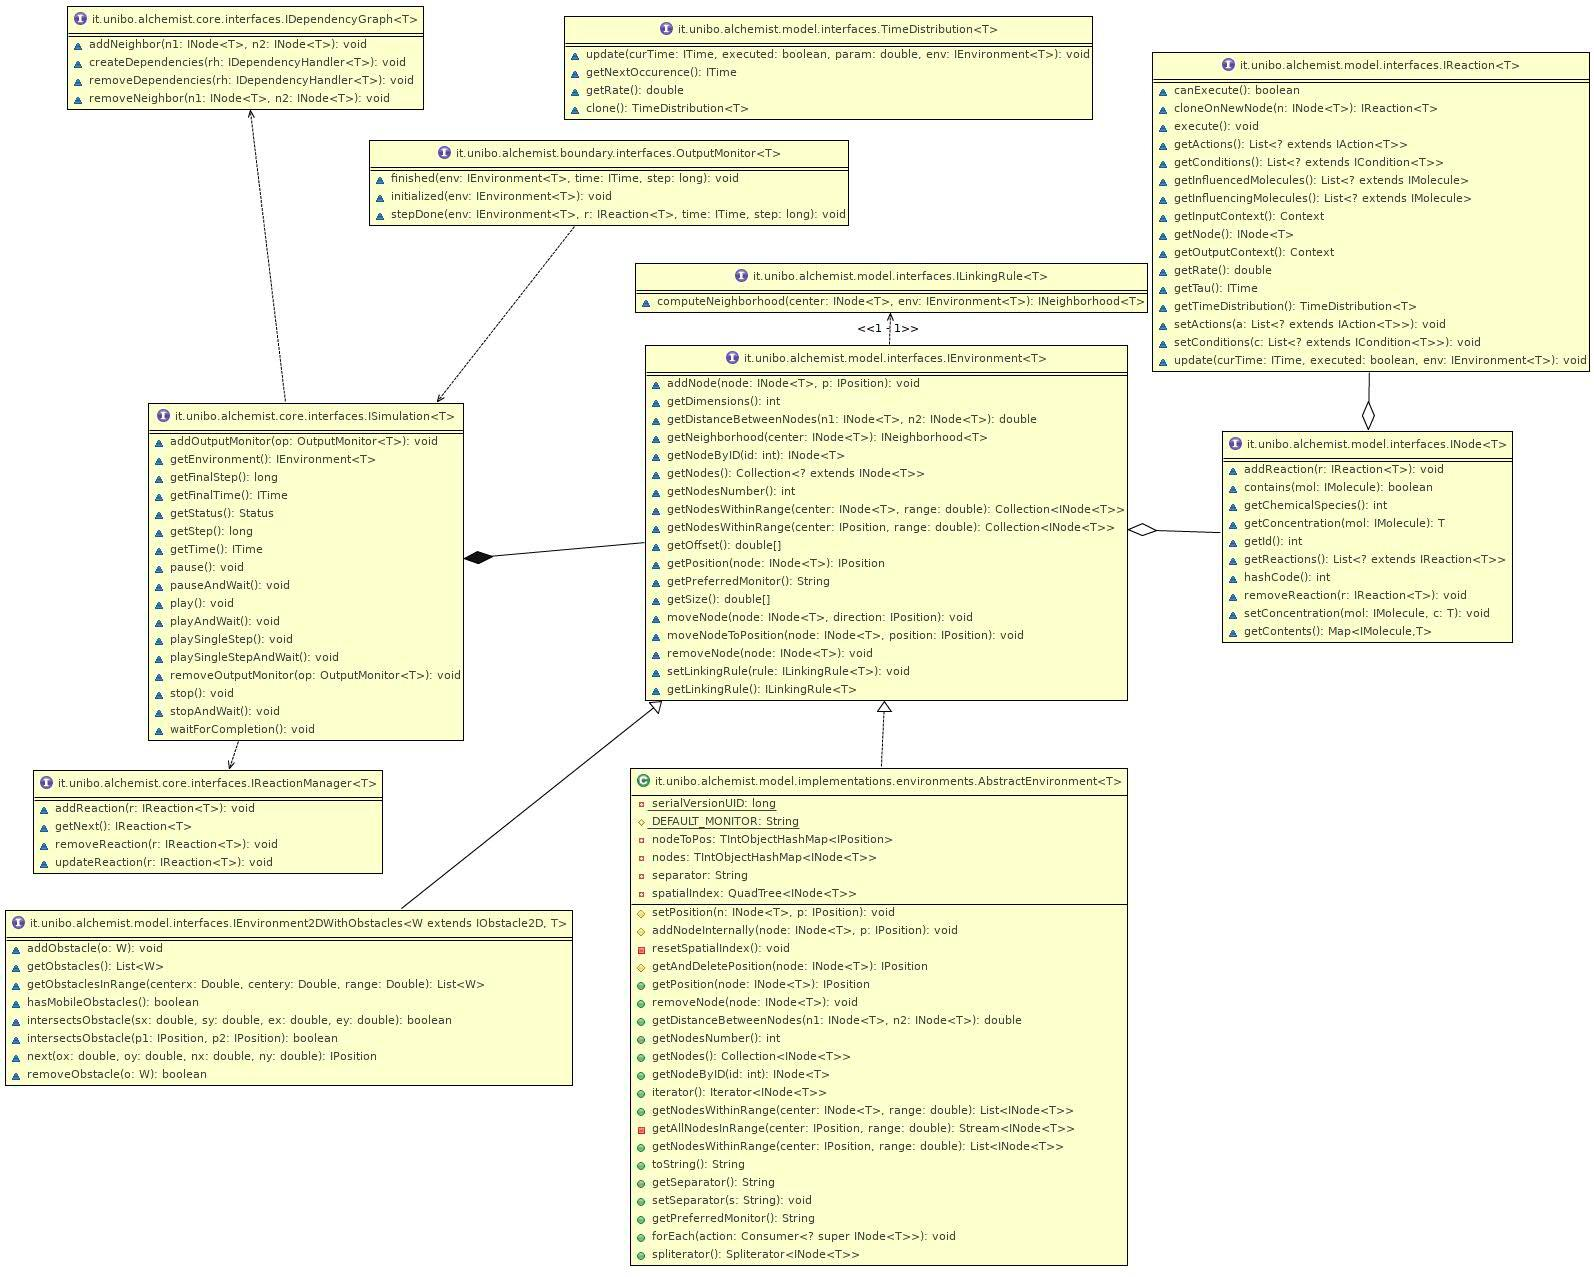
\includegraphics[width=\textwidth]{img/badarch}
\caption{Schema UML mal fatto e con una pessima descrizione, che non aiuta a capire. Don't try this at home.}
\label{img:badarch}
\end{figure}


\chapter{Sviluppo}
\section{Testing automatizzato}

Il testing automatizzato è un requisito di qualunque progetto software che si rispetti, e consente di verificare che non vi siano regressioni nelle funzionalità a fronte di aggiornamenti.
%
Per quanto riguarda questo progetto è considerato sufficiente un test minimale, a patto che sia completamente automatico.
%
Test che richiedono l'intervento da parte dell'utente sono considerati \textit{negativamente} nel computo del punteggio finale.

\subsection*{Elementi positivi}

\begin{itemize}
 \item Si descrivono molto brevemente i componenti che si è deciso di sottoporre a test automatizzato.
 \item Si utilizzano suite specifiche (e.g. JUnit) per il testing automatico.
\end{itemize}

\subsection*{Elementi negativi}
\begin{itemize}
 \item Non si realizza alcun test automatico.
 \item La non presenza di testing viene aggravata dall'adduzione di motivazioni non valide. Ad esempio, si scrive che l'interfaccia grafica non è testata automaticamente perché è \emph{impossibile} farlo\footnote{Testare in modo automatico le interfacce grafiche è possibile (si veda, come esempio, \url{https://github.com/TestFX/TestFX}), semplicemente nel corso non c'è modo e tempo di introdurvi questo livello di complessità. Il fatto che non vi sia stato insegnato come farlo non implica che sia impossibile!}.
 \item Si descrive un testing di tipo manuale in maniera prolissa.
 \item Si descrivono test effettuati manualmente che sarebbero potuti essere automatizzati, ad esempio scrivendo che si è usata l'applicazione manualmente.
 \item Si descrivono test non presenti nei sorgenti del progetto.
 \item I test, quando eseguiti, falliscono.
\end{itemize}

\section{Metodologia di lavoro}

Ci aspettiamo, leggendo questa sezione, di trovare conferma alla divisione operata nella sezione del design di dettaglio, e di capire come è stato svolto il lavoro di integrazione.
%
\textbf{Andrà realizzata una sotto-sezione separata per ciascuno studente} che identifichi le porzioni di progetto sviluppate, separando quelle svolte in autonomia da quelle sviluppate in collaborazione.
%
Diversamente dalla sezione di design, in questa è consentito elencare package/classi, se lo studente ritiene sia il modo più efficace di convogliare l'informazione.
%
Si ricorda che l'impegno deve giustificare circa 40-50 ore di sviluppo (è normale e fisiologico che approssimativamente la metà del tempo sia impiegata in analisi e progettazione).

\subsection*{Elementi positivi}

\begin{itemize}
	\item Si identifica con precisione il ruolo di ciascuno all'interno del gruppo, ossia su quale parte del progetto ciascuno dei componenti si è concentrato maggiormente.
	\item La divisione dei compiti è equa, ossia non vi sono membri del gruppo che hanno svolto molto più lavoro di altri.
	\item La divisione dei compiti è coerente con quanto descritto nelle parti precedenti della relazione.
	\item La divisione dei compiti è realistica, ossia le dipendenze fra le parti sviluppate sono minime.
	\item Si identifica quale parte del software è stato sviluppato da tutti i componenti insieme.
	\item Si spiega in che modo si sono integrate le parti di codice sviluppate separatamente, evidenziando eventuali problemi. Ad esempio, una strategia è convenire sulle interfacce da usare (ossia, occuparsi insieme di stabilire l'architettura) e quindi procedere indipendentemente allo sviluppo di parti differenti. Una possibile problematica potrebbe essere una dimenticanza in fase di design architetturale che ha costretto ad un cambio e a modifiche in fase di integrazione. Una situazione simile è la norma nell'ingegneria di un sistema software non banale, ed il processo di progettazione top-down con raffinamento successivo è il così detto processo ``a spirale''.
	\item Si descrive in che modo è stato impiegato il DVCS.
\end{itemize}

\subsection*{Elementi negativi}
\begin{itemize}
	\item Non si chiarisce chi ha fatto cosa.
	\item C'è discrepanza fra questa sezione e le sezioni che descrivono il design dettagliato.
	\item Tutto il progetto è stato svolto lavorando insieme invece che assegnando una parte a ciascuno.
	\item Non viene descritta la metodologia di integrazione delle parti sviluppate indipendentemente.
	\item Uso superficiale del DVCS.
\end{itemize}

\section{Note di sviluppo}

Questa sezione, come quella riguardante il design dettagliato va svolta \textbf{singolarmente da ogni membro del gruppo}.
%
Nella prima parte, ciascuno dovrà mostrare degli esempi di codice particolarmente ben realizzati,
che dimostrino proefficienza con funzionalità avanzate del linguaggio e capacità di spingersi oltre le librerie mostrate a lezione.

\begin{itemize}
	\item \textbf{Elencare} (fare un semplice elenco per punti, non un testo!) le feature \textit{avanzate} del linguaggio e dell'ecosistema Java che sono state
utilizzate. Le feature di interesse sono:
	\begin{itemize}
		\item Progettazione con generici, ad esempio costruzione di nuovi tipi generici, e uso di generici bounded.
		L'uso di classi generiche di libreria non è considerato avanzato.
		\item Uso di lambda expressions
		\item Uso di \texttt{Stream}, di \texttt{Optional} o di altri costrutti funzionali
		\item Uso di reflection
		\item Definizione ed uso di nuove annotazioni
		\item Uso del Java Platform Module System
		\item Uso di parti della libreria JDK non spiegate a lezione (networking, compressione, parsing XML, eccetera...)
		\item Uso di librerie di terze parti (incluso JavaFX): Google Guava, Apache Commons...
	\end{itemize}
	\item Si faccia molta attenzione a non scrivere banalità, elencando qui features di tipo ``core'', come le eccezioni, le enumerazioni, o le inner class: nessuna di queste è considerata avanzata.
	\item Per ogni feature avanzata, mostrata, includere:
	\begin{itemize}
		\item Nome della feature
		\item Permalink GitHub al punto nel codice in cui è stata utilizzata
	\end{itemize}
\end{itemize}

In questa sezione, \textit{dopo l'elenco},
vanno menzionati ed attributi con precisione eventuali pezzi di codice ``riadattati'' (o scopiazzati...) da Internet o da altri progetti,
pratica che tolleriamo ma che non raccomandiamo.
%
Si rammenta agli studenti che non è consentito partire da progetti esistenti e procedere per modifiche successive.
%
Si ricorda anche che i docenti hanno in mano strumenti antiplagio piuttosto raffinati e che ``capiscono'' il codice e la storia delle modifiche del progetto,
per cui tecniche banali come cambiare nomi (di classi, metodi, campi, parametri, o variabili locali),
aggiungere o togliere commenti,
oppure riordinare i membri di una classe vengono individuate senza problemi.
%
Le regole del progetto spiegano in dettaglio l'approccio dei docenti verso atti gravi come il plagiarismo.

I pattern di design \textbf{non} vanno messi qui.
%
L'uso di pattern di design (come suggerisce il nome) è un aspetto avanzato di design, non di implementazione,
e non va in questa sezione.

\subsection*{Elementi positivi}

\begin{itemize}
	\item Si elencano gli aspetti avanzati di linguaggio che sono stati impiegati
	\item Si elencano le librerie che sono state utilizzate
	\item Per ciascun elemento, si fornisce un permalink
	\item Ogni permalink fa riferimento ad uno snippet di codice scritto dall'autore della sezione (i docenti verificheranno usando \texttt{git blame})
	\item Se si è utilizzato un particolare algoritmo, se ne cita la fonte originale.
	Ad esempio, se si è usato Mersenne Twister per la generazione di numeri pseudo-random, si cita \cite{mersenne}.
	\item Si identificano parti di codice prese da altri progetti, dal web, o comunque scritte in forma originale da altre persone.
	In tal senso, si ricorda che agli ingegneri non è richiesto di re-inventare la ruota continuamente:
	se si cita debitamente la sorgente è tollerato fare uso di di snippet di codice open source per risolvere velocemente problemi non banali.
	Nel caso in cui si usino snippet di codice di qualità discutibile,
	oltre a menzionarne l'autore originale si invitano gli studenti ad adeguare tali parti di codice agli standard e allo stile del progetto.
	Contestualmente, si fa presente che è largamente meglio fare uso di una libreria che copiarsi pezzi di codice:
	qualora vi sia scelta (e tipicamente c'è), si preferisca la prima via.
\end{itemize}

\subsection*{Elementi negativi}
\begin{itemize}
	\item Si elencano feature core del linguaggio invece di quelle segnalate. Esempi di feature core da non menzionare sono:
    \begin{itemize}
        \item eccezioni;
        \item classi innestate;
        \item enumerazioni;
        \item interfacce.
    \end{itemize}
	\item Si elencano applicazioni di terze parti (peggio se per usarle occorre licenza, e lo studente ne è sprovvisto) che non c'entrano nulla con lo sviluppo, ad esempio:
    \begin{itemize}
        \item Editor di grafica vettoriale come Inkscape o Adobe Illustrator;
        \item Editor di grafica scalare come GIMP o Adobe Photoshop;
        \item Editor di audio come Audacity;
        \item Strumenti di design dell'interfaccia grafica come SceneBuilder: il codice è in ogni caso inteso come sviluppato da voi.
    \end{itemize}
	\item Si descrivono aspetti di scarsa rilevanza, o si scende in dettagli inutili.
	\item Sono presenti parti di codice sviluppate originalmente da altri che non vengono debitamente segnalate.
	In tal senso, si ricorda agli studenti che i docenti hanno accesso a tutti i progetti degli anni passati,
	a Stack Overflow,
	ai principali blog di sviluppatori ed esperti Java,
	ai blog dedicati allo sviluppo di soluzioni e applicazioni
	(inclusi blog dedicati ad Android e allo sviluppo di videogame),
	nonché ai vari GitHub, GitLab, e Bitbucket.
	Conseguentemente, è \emph{molto} conveniente \emph{citare} una fonte ed usarla invece di tentare di spacciare per proprio il lavoro di altri.
	\item Si elencano design pattern
\end{itemize}

\subsection{Esempio}

\subsubsection{Utilizzo della libreria SLF4J}

Utilizzata in vari punti.
Un esempio è \url{https://github.com/AlchemistSimulator/Alchemist/blob/5c17f8b76920c78d955d478864ac1f11508ed9ad/alchemist-swingui/src/main/java/it/unibo/alchemist/boundary/swingui/effect/impl/EffectBuilder.java#L49}

\subsubsection{Utilizzo di \texttt{LoadingCache} dalla libreria Google Guava}

Permalink: \url{https://github.com/AlchemistSimulator/Alchemist/blob/d8a1799027d7d685569e15316a32e6394632ce71/alchemist-incarnation-protelis/src/main/java/it/unibo/alchemist/protelis/AlchemistExecutionContext.java#L141-L143}

\subsubsection{Utilizzo di \texttt{Stream} e lambda expressions}

Usate pervasivamente. Il seguente è un singolo esempio.
Permalink: \url{https://github.com/AlchemistSimulator/Alchemist/blob/d8a1799027d7d685569e15316a32e6394632ce71/alchemist-incarnation-protelis/src/main/java/it/unibo/alchemist/model/ProtelisIncarnation.java#L98-L120}

\subsubsection{Scrittura di metodo generico con parametri contravarianti}

Permalink: \url{https://github.com/AlchemistSimulator/Alchemist/blob/d8a1799027d7d685569e15316a32e6394632ce71/alchemist-incarnation-protelis/src/main/java/it/unibo/alchemist/protelis/AlchemistExecutionContext.java#L141-L143}

\subsubsection{Protezione da corse critiche usando \texttt{Semaphore}}

Permalink: \url{https://github.com/AlchemistSimulator/Alchemist/blob/d8a1799027d7d685569e15316a32e6394632ce71/alchemist-incarnation-protelis/src/main/java/it/unibo/alchemist/model/ProtelisIncarnation.java#L388-L440}


\chapter{Commenti finali}

In quest'ultimo capitolo si tirano le somme del lavoro svolto e si delineano eventuali sviluppi
futuri.

\textit{Nessuna delle informazioni incluse in questo capitolo verrà utilizzata per formulare la valutazione finale}, a meno che non sia assente o manchino delle sezioni obbligatorie.
%
Al fine di evitare pregiudizi involontari, l'intero capitolo verrà letto dai docenti solo dopo aver formulato la valutazione.

\section{Autovalutazione e lavori futuri}

\textbf{È richiesta una sezione per ciascun membro del gruppo, obbligatoriamente}.
%
Ciascuno dovrà autovalutare il proprio lavoro, elencando i punti di forza e di debolezza in quanto prodotto.
Si dovrà anche cercare di descrivere \emph{in modo quanto più obiettivo possibile} il proprio ruolo all'interno del gruppo.
Si ricorda, a tal proposito, che ciascuno studente è responsabile solo della propria sezione: non è un problema se ci sono opinioni contrastanti, a patto che rispecchino effettivamente l'opinione di chi le scrive.
Nel caso in cui si pensasse di portare avanti il progetto, ad esempio perché effettivamente impiegato, o perché sufficientemente ben riuscito da poter esser usato come dimostrazione di esser capaci progettisti, si descriva brevemente verso che direzione portarlo.

\section{Difficoltà incontrate e commenti per i docenti}

Questa sezione, \textbf{opzionale}, può essere utilizzata per segnalare ai docenti eventuali problemi o difficoltà incontrate nel corso o nello svolgimento del progetto, può essere vista come una seconda possibilità di valutare il corso (dopo quella offerta dalle rilevazioni della didattica) avendo anche conoscenza delle modalità e delle difficoltà collegate all'esame, cosa impossibile da fare usando le valutazioni in aula per ovvie ragioni.
%
È possibile che alcuni dei commenti forniti vengano utilizzati per migliorare il corso in futuro: sebbene non andrà a vostro beneficio, potreste fare un favore ai vostri futuri colleghi.
%
Ovviamente \textit{il contenuto della sezione non impatterà il voto finale}.

\appendix
\chapter{Guida utente}

Capitolo in cui si spiega come utilizzare il software. Nel caso in cui il suo uso sia del tutto
banale, tale capitolo può essere omesso.
%
A tal riguardo, si fa presente agli studenti che i docenti non hanno mai utilizzato il software
prima, per cui aspetti che sembrano del tutto banali a chi ha sviluppato l'applicazione possono non
esserlo per chi la usa per la prima volta.
%
Se, ad esempio, per cominciare una partita con un videogioco è necessario premere la barra
spaziatrice, o il tasto ``P'', è necessario che gli studenti lo segnalino.

\subsection*{Elementi positivi}

\begin{itemize}
 \item Si istruisce in modo semplice l'utente sull'uso dell'applicazione, eventualmente facendo uso di schermate e descrizioni.
\end{itemize}

\subsection*{Elementi negativi}
\begin{itemize}
 \item Si descrivono in modo eccessivamente minuzioso tutte le caratteristiche, anche minori, del software in oggetto.
 \item Manca una descrizione che consenta ad un utente qualunque di utilizzare almeno le funzionalità primarie dell'applicativo.
\end{itemize}

\chapter{Esercitazioni di laboratorio}

In questo capitolo ciascuno studente elenca gli esercizi di laboratorio che ha svolto
(se ne ha svolti),
elencando i permalink dei post sul forum dove è avvenuta la consegna.
%
Questa sezione potrebbe essere processata da strumenti automatici,
per cui link a oggetti diversi dal permalink della consegna,
errori nell'email o nel nome del laboratorio possono portare ad ignorare alcune consegne,
si raccomanda la massima precisione.

\section*{Esempio}

\subsection{paolino.paperino@studio.unibo.it}

\begin{itemize}
 \item Laboratorio 04: \url{https://virtuale.unibo.it/mod/forum/discuss.php?d=12345#p123456}
 \item Laboratorio 06: \url{https://virtuale.unibo.it/mod/forum/discuss.php?d=22222#p222222}
 \item Laboratorio 09: \url{https://virtuale.unibo.it/mod/forum/discuss.php?d=99999#p999999}
\end{itemize}

\subsection{paperon.depaperoni@studio.unibo.it}

\begin{itemize}
 \item Laboratorio 04: \url{https://virtuale.unibo.it/mod/forum/discuss.php?d=12345#p123456}
 \item Laboratorio 05: \url{https://virtuale.unibo.it/mod/forum/discuss.php?d=22222#p222222}
 \item Laboratorio 06: \url{https://virtuale.unibo.it/mod/forum/discuss.php?d=99999#p999999}
 \item Laboratorio 07: \url{https://virtuale.unibo.it/mod/forum/discuss.php?d=22222#p222222}
 \item Laboratorio 08: \url{https://virtuale.unibo.it/mod/forum/discuss.php?d=99999#p999999}
 \item Laboratorio 09: \url{https://virtuale.unibo.it/mod/forum/discuss.php?d=22222#p222222}
 \item Laboratorio 10: \url{https://virtuale.unibo.it/mod/forum/discuss.php?d=99999#p999999}
 \item Laboratorio 11: \url{https://virtuale.unibo.it/mod/forum/discuss.php?d=22222#p222222}
\end{itemize}


\bibliographystyle{alpha}
\bibliography{13-template}

\end{document}
